\documentclass[10pt]{article}
\usepackage{authblk}
\usepackage{amsmath}
\usepackage[margin=1.2in]{geometry}
\usepackage{listings}
\usepackage{caption}
\usepackage{graphicx}
\usepackage[titletoc,title]{appendix}
\usepackage{float}
\usepackage[hidelinks]{hyperref}
\floatstyle{boxed}
\restylefloat{figure}

\title{\bf Simple Game Solving Using Haskell}
\author{Daniel Leblanc}
\date{March 25, 2014}

\begin{document}
\maketitle

\section{Introduction}
\paragraph{} A solved game is one for which, if we assume both players play perfectly,
    the outcome is known.  Many games are much too complicated to completely explore
    the possible game states.  Games such as Chess and Go have too many 
    possible moves from each board position to ever be able to fully explore without 
    vastly superior computing power to what is now available.  To give you an idea 
    of the potential complexity, Checkers, which is the most complicated game to be
    solved to date, has 500 billion billion possible board positions $(5 \times 10^{20})$
    \cite{checkersSolved} and took nearly two decades of constant processing to solve. 
\paragraph{} The vast majority of
    two player games can be mapped to decision problems that are PSPACE-complete.  This
    puts them in a category of problems that are at least as difficult to solve as 
    NP-complete problems.  Despite this some simpler games have small enough game trees
    that we can fully explore them in reasonable amounts of time.
\paragraph{} Here we experiment with implementing a game solver in Haskell for several 
    simple two player games.  Haskell is an excellent choice when exploring a complete 
    game tree, as it allows us to avoid the traditionally tedious task of rewinding 
    the board positions after each move.
\paragraph{} All code for the project is available at my github account, 
    \url{https://github.com/crophix/GameSolver}, as well as in the appendices.

\section{Adversarial Search}
\paragraph{} Adversarial search is a branch of artificial intelligence that attempts to 
    create optimal players for various games.  It creates a tree of possible moves and 
    then searches the game tree looking for the best possible sequence of moves.  The 
    algorithm we are using here is called $negamax$ and looks for the worst move for 
    the opponent at each step in the search.  Figure \ref{negamaxpseudo} shows some
    simple pseudocode.  In more complex games each board position needs to be scored
    even if it isn't a final game state.  For our purposes we only score boards when 
    the game is in a termination state, since we are not trying to produce an optimal
    player, just solve the game assuming optimal play.  This allows us to not limit 
    our running time to human patience, and instead completely explore the game tree.

\begin{figure}[ht]
    \centering
    \begin{verbatim}
    negamax(g)
        if g is a final state (game over)
            return the value of g
        v <- -1
        for each legal move m in g
            g' <- m(g)
            v' <- -negamax(g')
            if v' > v
                v <- v'
        return v \end{verbatim}
    \caption{Pseudocode for negamax search} \label{negamaxpseudo}
\end{figure}

\paragraph{} There are several optimizations that can be done to improve the performance 
    of negamax search such as $alpha-beta$ pruning and limiting the depth of the search that we have 
    ignored for our initial implementation, but could easily be added later.  Further 
    improvements can also be made by taking into account board rotations and translations 
    to reduce the size of the potential game tree.  This however would take significant 
    additional work and has been ignored for this paper.
    
\paragraph{} In Haskell $negamax$ has been implemented as a higher order function as seen 
    in figure \ref{haskellnegamax}.  It takes three functions and a game state as input 
    and returns an integer value.  If optimal play would result in the currently active 
    player winning the integer is positive, negative if the active player has no way to 
    prevent a loss, and zero if optimal play would result in a draw.  The first function 
    just determines if the current position is a final state.  The second function 
    produces a list of all possible game states that can be reached from the current 
    position in one move.  The final function produces the score if the game is over.
    Using $map$ and $maximum$ we can avoid the loop seen in figure \ref{negamaxpseudo}.

\begin{figure}[ht]
    \centering
    \begin{verbatim}
    negamax    :: (a -> Bool) -> (a -> [a]) -> (a -> Int) -> a -> Int
    egamax over moves eval game 
               | over game = eval game
               | otherwise = maximum (map 
                               (negate . (negamax over moves eval)) 
                               (moves game)) \end{verbatim}
\caption{Haskell implementation of negamax search} \label{haskellnegamax}
\end{figure}

\paragraph{} The negamax implementation was incorporated into a module that other games
    can then include. This allows anything that implements the required set of functions
    to use the same negamax search.  The implementation I use could likely be simplified 
    further by removing the check for final state and using a Maybe value in one of the 
    other functions.  Implementing a type class that restricts the type of $a$ might also
    be good idea, but has been ignored at present.

\section{Tic-Tac-Toe}
\subsection{Description}
    \paragraph{} Tic-Tac-Toe, also known as Noughts and Crosses or Xs and Os, is a 
        simple paper and pencil game for two players, who take turns marking the 
        spaces on a $3 \times 3$ grid.  The player who succeeds in placing three marks
        in row is the winner.  The game is mostly common with younger children as 
        most people quickly realize that optimal play will always result in a draw.
    \paragraph{} Despite the simple nature of the game, Tic-Tac-Toe has 255,168 possible
        game states \cite{tttnosym} if we ignore any possible symmetries.  Which is not
        an insignificant search space.  Taking symmetries into account would reduce the
        number of possible state to only 26,830 \cite{tttsym}, which is much smaller, 
        but identifying symmetry would likely cost us significant computation time.

\subsection{Haskell Implementation}
    \paragraph{} To begin I created two data types to track the game state, shown in 
    figure \ref{hasktttgame}.  The first keeps track of information regarding a single
    square.  The square may contain an X or an O, or it may be empty, in which case I 
    keep track of an integer associated with it's location.  Because I will often
    need to compare or display squares I am deriving Eq and Show.  The exact game 
    state is represented by the TicTacToe data type, which stores the game board and
    the Symbol of the player on move.  I don't specify the size of the board here, so
    I can easy expand this for use on larger game boards.

    \begin{figure}[ht]
        \centering
        \begin{verbatim}
    data Symbol    = Empty Int | X | O deriving (Eq, Show)
    data TicTacToe = Game { board :: [[Symbol]], onMove :: Symbol }\end{verbatim}
        \caption{Tic-Tac-Toe representation in Haskell} \label{hasktttgame}
    \end{figure}

    \paragraph{} A game of Tic-Tac-Toe ends when either a player has won or when 
    there are no available moves.  The functions shown in figure \ref{tttover} check
    if the current state is a final state.  The gameOver and tieGame functions are
    self explanatory, but the wonGame function is a little more interesting.  It 
    creates a list of winning symbols.  In reality this list rarely contains more 
    than one symbol, and when it does, all symbols in the list are the same.  
    However, there are other variants of Tic-Tac-Toe that I might want to represent, 
    so I made the function a little more powerful than required.  The function checks
    to see if there is a row column or diagonal with all elements the same.  The rows
    and columns are easy to check, just using the original board for the rows and the
    transpose for the columns.  The diagonals are a little more interesting and are 
    checked just using an explicit list comprehension.  The downside of
    this implementation is it only works on a $3 \times 3$ board.  A larger board 
    would require extensive changes to the current implementation of the diag
    function.

    \begin{figure}[ht]
        \centering
        \begin{verbatim}
    gameOver  :: TicTacToe -> Bool
    gameOver g = (not $ null (wonGame g)) || tieGame g

    wonGame  :: TicTacToe -> [Symbol]
    wonGame g = [x | [x,y,z] <- lines, x == y && y == z]
                where diag [[a,_,b],
                            [_,c,_],
                            [d,_,e]] = [[a,c,e],[b,c,d]]
                      brd   = board g
                      lines = brd ++ diag brd ++ transpose brd

    tieGame :: TicTacToe -> Bool
    tieGame  = null . moves        \end{verbatim}
        \caption{Checking for game completion.} \label{tttover}
    \end{figure}

    \paragraph{} To create the list of possible game states that can be reach from the 
    current position on one move I created the functions shown in figure \ref{tttmoves}.
    The moves function just creates a list of all squares that aren't currently an X 
    or an O.  I then use that list to create a new list of game states where the 
    active player has marked each of the available squares.

    \begin{figure}[ht]
        \centering
        \begin{verbatim}
    applyMoves  :: TicTacToe -> [TicTacToe]
    applyMoves g | gameOver g = []
                 | otherwise  =[makeMove g s | s <- moves g]

    moves  :: TicTacToe -> [Symbol]
    moves g = [x | x <- concat (board g), x /= X, x /= O]
    
    makeMove    :: TicTacToe -> Symbol -> TicTacToe
    makeMove g s = Game (map (map place) (board g)) p
                   where p = switchPlayer (onMove g)
                         place b | b == s    = onMove g
                                 | otherwise = b        \end{verbatim}
        \caption{Creates a list of all possible game states that can be reached
        in one move.} \label{tttmoves}
    \end{figure}

    \paragraph{} Scoring a game of Tic-Tac-Toe was quite simple and the function I
    built can be seen in figure \ref{ttteval}.  A tie game is worth zero points and
    a winning position is worth three points to whoever has won.  The one point result
    isn't actually used anywhere in my program, but I wanted an option for including 
    limiting the search to a specified depth which would require a score for all possible 
    results.

    \begin{figure}[ht]
        \centering
        \begin{verbatim}
    gameEval  :: TicTacToe -> Int
    gameEval g | tieGame g               =  0
               | null winner             =  1
               | head winner == onMove g =  3
               | otherwise               = -3
                 where winner = wonGame g        \end{verbatim}
        \caption{Tic-Tac-Toe game evaluation} \label{ttteval}
    \end{figure}

    \paragraph{} As a final piece I turned the ascii art program we built for assignment
    three into a module and added code for displaying the board in a simple style.  The 
    code can be seen in figure \ref{tttascii}.  The main reason for including this was
    to verify everything is working correctly, as I can now create boards in several 
    different states where I know what the outcome should be and verify that my results 
    match.  The implementation just takes advantage of the align function written 
    previously to assemble the individual squares into the appropriate grid.

    \begin{figure}[ht]
        \centering
        \begin{verbatim}
    picGame       :: TicTacToe -> Pic
    picGame g      = picBoard (board g)       

    picBoard      :: [[Symbol]] -> Pic
    picBoard board = align center (map (align middle) b)
                     where b = map (map picSquare) board

    picSquare     :: Symbol -> Pic
    picSquare x    = align center [tope, align middle [edge, item,edge], tope]
                     where edge = text ["|","|","|"]
                           tope = string "+-----+"
                           item = string ("  " ++ (r x) ++ "  ")
                           r (Empty n) = show n
                           r a         = show x \end{verbatim}
        \caption{Ascii art display of the Tic-Tac-Toe board.} \label{tttascii}
    \end{figure}
 
\subsection{Results}
    \paragraph{} On Tic-Tac-Toe my results were exactly what was expected.  It explored
    the complete game tree in about twenty seconds when run from the interpreter on my home
    computer, and returned the expected result in all cases.  The starting board 
    position, displayed using the method shown in figure \ref{tttascii}, and the result
    from my negamax function are shown in figure \ref{tttcat}, figure \ref{tttX}, and 
    figure \ref{tttO}.

    \begin{figure}[ht]
        \centering
        \begin{verbatim}
            *Main> render (picGame initialState)
            +-----++-----++-----+
            |     ||     ||     |
            |  1  ||  2  ||  3  |
            |     ||     ||     |
            +-----++-----++-----+
            +-----++-----++-----+
            |     ||     ||     |
            |  4  ||  5  ||  6  |
            |     ||     ||     |
            +-----++-----++-----+
            +-----++-----++-----+
            |     ||     ||     |
            |  7  ||  8  ||  9  |
            |     ||     ||     |
            +-----++-----++-----+
            *Main> negamax initialState 
            0    \end{verbatim}
        \caption{Negamax starting with the empty board.  Expected result: 0}\label{tttcat}
    \end{figure}

    \begin{figure}[ht]
        \centering
        \begin{verbatim}
            *Main> render (picGame testState1)
            +-----++-----++-----+
            |     ||     ||     |
            |  1  ||  O  ||  3  |
            |     ||     ||     |
            +-----++-----++-----+
            +-----++-----++-----+
            |     ||     ||     |
            |  4  ||  X  ||  6  |
            |     ||     ||     |
            +-----++-----++-----+
            +-----++-----++-----+
            |     ||     ||     |
            |  7  ||  8  ||  9  |
            |     ||     ||     |
            +-----++-----++-----+
            *Main> negamax testState1
            3    \end{verbatim}
        \caption{Negamax starting with X having the advantage. Expected result: 3}\label{tttX}
    \end{figure}

    \begin{figure}[ht]
        \centering
        \begin{verbatim}
            *Main> render (picGame testState2)
            +-----++-----++-----+
            |     ||     ||     |
            |  O  ||  X  ||  3  |
            |     ||     ||     |
            +-----++-----++-----+
            +-----++-----++-----+
            |     ||     ||     |
            |  4  ||  O  ||  6  |
            |     ||     ||     |
            +-----++-----++-----+
            +-----++-----++-----+
            |     ||     ||     |
            |  7  ||  X  ||  9  |
            |     ||     ||     |
            +-----++-----++-----+
            *Main> negamax testState2
            -3    \end{verbatim}
        \caption{Negamax starting with O having the advantage.  Expected result: -3}\label{tttO}
    \end{figure}

    \paragraph{} I was really quite pleased with the overall end result of the 
    Tic-Tac-Toe program.  The speed was reasonable, and might be improved by 
    adding a main function so that I can compile the code before running.  It also
    successfully solves some of the more obscure game states that humans often 
    get incorrect.  Some speed increases would be needed if I wanted to include 
    this in an interactive Tic-Tac-Toe game, but not an excessive amount.  This
    code was the first I finished and I was excited to move onto trying to solve
    a more complicated game.

\clearpage
\section{Fox and Hounds}
\subsection{Description}
    \paragraph{} The game Fox and Hounds has also been known as Wolf and Sheep, 
    Hounds and Hares, or Devil and Tailors.  It is played on an $8 \times 8$
    checkers or chess board and is somewhat unusual in that the two teams are 
    mismatched.  As in checkers, only the dark squares are used and pieces
    only move diagonally.  The Hounds player begins with four pieces starting 
    at their board edge and may move diagonally only forwards.  The Fox player 
    starts with a single piece and may move diagonally forwards and backwards.
    Unlike checkers no jumps or captures may be made.  A typical starting position
    is shown in figure \ref{foxHoundspng}.  The goal of the Hounds is to corner the
    Fox in a position where it can no longer move.  The goal of the Fox is to 
    reach the starting position of one of the Hounds.

    \paragraph{} Fox and Hounds was solved in 1982 \cite{winningWays} and was 
    found to be a Hounds victory when played perfectly.  The game was not solved 
    by exploring the game tree, instead Berlekamp, Conway and Guy devised a 
    winning strategy that could respond to any possible move by the Fox.
    Unlike Tic-Tac-Toe this game has an extremely large game tree that
    needs to be searched.  This proved to be much more difficult than the 
    solving Tic-Tac-Toe.

\floatstyle{plain}
\restylefloat{figure}
    \begin{figure}[ht]
        \centering
        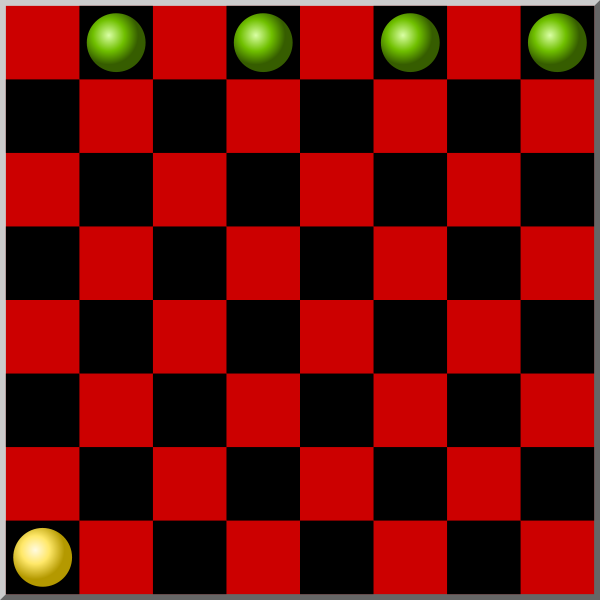
\includegraphics[width=5cm]{foxHounds.png}
        \caption{Typical starting positions for Fox and Hounds} \label{foxHoundspng}
    \end{figure}
\floatstyle{boxed}
\restylefloat{figure}


\subsection{Haskell Implementation}
    \paragraph{} To track the game state of Fox and Hounds I creates two data types
    just like for Tic-Tac-Toe.  The code is shown in figure \ref{haskhhgame}.
    Each square on the board has a location, which is 
    represented by a tuple of integers and is either empty or contains a piece.
    A complete game state is a list of squares, a player on move, and the positions 
    of all of the pieces.  Unlike in Tic-Tac-Toe I chose to represent the positions 
    of all the pieces separately in addition to their location on the board.  This 
    allowed me to check for winning game states and available moves much 
    more easily.  Keeping track of the positions on the board allowed me to display
    the game more easily as well.  I also store the allowed moves for each of the 
    pieces since the two sides move differently.

    \begin{figure}[ht]
        \centering
        \begin{verbatim}
    type Position   = (Int, Int)
    type Moves      = [(Int, Int)]
    data Symbol     = Empty | H | F deriving (Eq, Show)
    data FoxHounds  = Game { board  :: [(Position,Symbol)],
                             onMove :: Symbol,
                             hounds :: [Position],
                             fox    :: Position}

    foxMoves   :: Moves --Diagonal in any direction
    foxMoves    = [(-1,-1),(1,-1),(-1,1),(1,1)]
    houndMoves :: Moves --Diagonal forward only
    houndMoves  = [(1,-1),(1,1)]        \end{verbatim}
        \caption{Fox and Hounds representation in Haskell} \label{haskhhgame}
    \end{figure}

    \paragraph{} My initial attempts at recognizing a final game state only took into
    account the two possible winning conditions.  Recognizing when the fox has no 
    available moves is easy enough, as is recognizing when the fox is in a winning
    position.  The third possibility is that the hounds have no available moves, but
    the fox is not yet in a winning position.  In traditional play, the hounds would 
    lose a turn and the fox would get a chance to move again, but because I was already
    having issues with the size of the game tree I chose to represent this as a final
    state.  My implementation is shown in figure \ref{hhover} and takes heavy advantage
    null to recognize the various positions.

    \begin{figure}[ht]
        \centering
        \begin{verbatim}
    gameOver  :: FoxHounds -> Bool
    gameOver g = null (moves (fox g) (hounds g) foxMoves) || 
                 (and $ map null [moves s [fox g] houndMoves | s <- hounds g]) ||
                 fst (fox g) == 1        \end{verbatim}
        \caption{Checking for game completion.} \label{hhover}
    \end{figure}

    \paragraph{} Unlike Tic-Tac-Toe, where creating the list of moves was quite
    simple, Fox and Hounds requires significant work to accurately represent all
    game states that can be reached in one move.  The functions shown in figure 
    \ref{hhmoves} were created for this purpose.  The moves function creates a list of
    all positions that can be reached from a given location, using one of the defined 
    movement patterns shown in figure \ref{haskhhgame}.  All moves are checked to 
    make sure they are still on the board and not currently occupied by another piece.
    The applyMove function generates a new game state with a piece moved from the 
    starting position to the ending position.  The final function, allMoves, just 
    used a list comprehension and the previous two functions to create a list
    of all states that can be reach from the present position.

    \begin{figure}[ht]
        \centering
        \begin{verbatim}
    allMoves  :: FoxHounds -> [FoxHounds]
    allMoves g | onMove g == H = [applyMove g s e | s <- hounds g, 
                                    e <- moves s (fox g : hounds g) houndMoves]
               | otherwise     = [applyMove g (fox g) e | 
                                    e <- moves (fox g) (hounds g) foxMoves]

    moves           :: Position -> [Position] -> Moves -> [(Int, Int)]
    moves (a,b) o ms = [(a+x, b+y) | (x,y) <- ms, 
                                     a+x > 0 && a+x < 9,
                                     b+y > 0 && b+y < 9, 
                                     not ((a+x,b+y) `elem` o)]

    applyMove  :: FoxHounds -> Position -> Position -> FoxHounds
    applyMove g start end
                = Game (map (clear . place) (board g)) (switchPlayer $ onMove g) h f
                  where clear a | fst a == start = (start,Empty)
                                | otherwise      = a
                        place a | fst a == end   = (end, onMove g)
                                | otherwise      = a
                        h | onMove g == H = end : [x | x <- hounds g, x /= start]
                          | otherwise     = hounds g
                        f | onMove g == F = end
                          | otherwise     = fox g        \end{verbatim}
        \caption{Creates a list of all possible game states that can be reached
        in one move.} \label{hhmoves}
    \end{figure}

    \paragraph{} The function for scoring a game can be seen in figure \ref{hheval}
    and is quite simple.  If the fox has no available moves, then the hounds have won,
    and if the fox has reach the first row, the fox has won.  All other cases are 
    treated as a draw.

    \begin{figure}[ht]
        \centering
        \begin{verbatim}
    scoreGame  :: FoxHounds -> Int
    scoreGame g | null (moves (fox g) (hounds g) foxMoves) =  p
                | fst (fox g) == 1                         = -p
                | otherwise                                =  0
                  where p | onMove g == H =  1
                          | otherwise     = -1        \end{verbatim}
        \caption{Fox and hounds game evaluation} \label{hheval}
    \end{figure}

    \paragraph{} Once again I used the Ascii art program written previously to display
    the game board for testing purposes.  The code can be seen in figure \ref{hhascii}.
    This was also significantly more challenging than displaying the Tic-Tac-Toe board.
    Each square is responsible for displaying it's contents as well as it's top and left
    edges.  Squares that are available to be moved through are shown empty and squares
    which are off limits are filled with '\#'.  Since the board in this case is stored
    as a single list instead of a list of lists, I needed a way to split the list every
    eight squares.  I used splitEvery to do this, which I took from the $Data.List.Split$
    library.  The code is included here for convenience.

    \begin{figure}[ht]
        \centering
        \begin{verbatim}
    picGame   :: FoxHounds -> Pic
    picGame g  = picBoard (board g)

    picSquare          :: (Position,Symbol) -> Pic
    picSquare ((a,b),x) = align center [tope, align middle [edge, item]]
                          where edge = text ["|"]
                                tope = string "+---"
                                item = string (r x)
                                r Empty | even (a+b) = "   "
                                        | odd  (a+b) = "###"
                                r t                  = " " ++ show x ++ " "

    picBoard   :: [(Position,Symbol)] -> Pic
    picBoard ps = align center ([picRow x | x <- splitEvery 8 ps] ++ 
                                [string "+---+---+---+---+---+---+---+---+"])

    picRow ps = align middle ((map picSquare ps) ++ [text ["+","|"]])

    splitEvery     :: Int -> [a] -> [[a]]
    splitEvery i ls = map (take i) (build (splitter ls))
                      where splitter [] _ n = n
                            splitter l c n  = l `c` splitter (drop i l) c n
                            build g         = g (:) []    \end{verbatim}
        \caption{Ascii art for the Fox and Hounds game.} \label{hhascii}
    \end{figure}
 
\clearpage
\subsection{Results}
    \paragraph{} Here's where my success starts to wane a bit.  My representation 
    correctly solves simpler game states but is quite slow even on those instances.
    Solving the complete game tree would take longer than I have patience for.  
    Even with 24 hours of continuous processing I still hadn't reached a final state.
    While everything certainly seems to work for simple cases, I can't explicitly
    guarantee that it works for solving the complete game.  Figures \ref{hwin} and
    \ref{fwin} show the results from running on some simpler game states.

    \begin{figure}[ht]
        \centering
        \begin{verbatim}
            *Main> render (picGame tState1)
            +---+---+---+---+---+---+---+---+
            |   |###|   |###|   |###|   |###|
            +---+---+---+---+---+---+---+---+
            |###|   |###|   |###|   |###|   |
            +---+---+---+---+---+---+---+---+
            |   |###|   |###|   |###|   |###|
            +---+---+---+---+---+---+---+---+
            |###|   |###|   |###|   |###|   |
            +---+---+---+---+---+---+---+---+
            |   |###|   |###| H |###| H |###|
            +---+---+---+---+---+---+---+---+
            |###|   |###|   |###|   |###|   |
            +---+---+---+---+---+---+---+---+
            |   |###|   |###| H |###|   |###|
            +---+---+---+---+---+---+---+---+
            |###|   |###| H |###|   |###| F |
            +---+---+---+---+---+---+---+---+
            *Main> negamax tState1 
            -1    \end{verbatim}
        \caption{Solved game with Hounds having the advantage.} \label{hwin}
    \end{figure}

    \begin{figure}[ht]
     \centering
        \begin{verbatim}
            *Main> render (picGame tState2)
            +---+---+---+---+---+---+---+---+
            | H |###|   |###|   |###|   |###|
            +---+---+---+---+---+---+---+---+
            |###|   |###|   |###|   |###|   |
            +---+---+---+---+---+---+---+---+
            |   |###|   |###|   |###|   |###|
            +---+---+---+---+---+---+---+---+
            |###|   |###|   |###|   |###|   |
            +---+---+---+---+---+---+---+---+
            |   |###|   |###|   |###|   |###|
            +---+---+---+---+---+---+---+---+
            |###|   |###|   |###|   |###| F |
            +---+---+---+---+---+---+---+---+
            |   |###|   |###|   |###| H |###|
            +---+---+---+---+---+---+---+---+
            |###|   |###| H |###| H |###|   |
            +---+---+---+---+---+---+---+---+
            *Main> negamax tState2
            1    \end{verbatim}
        \caption{Solved game with Fox having the advantage.} \label{fwin}
    \end{figure}

\section{Future Work}
\paragraph{} There are several task I would have liked to have gotten to that I 
just didn't get a chance to finish.  There are several improvements that can be 
made to the negamax search algorithm that would significantly improve the running 
time.  I also started implementing a solver for a third game, but was unable to 
complete it in time for the report.

\paragraph{} The game Quantum Tic-Tac-Toe is a variant on the tradition game where 
each player takes turns marking two squares which are superpositions of eachother.
The game was developed by Alan Goff as a teaching aid for students trying to 
understand quantum superpositions \cite{qtttdesign} and adds an interesting 
additional dimension to the game.  The game was solved in January of 2011 by
Ishizeki and Matsuura \cite{qtttsolved}.  I've previously written a solver for the 
game in Python, but I couldn't figure out an efficient way to find the quantum 
entanglements in Haskell.  I should be able to get my solution working with another
couple days worth of work, but at this point the representation isn't complete.

\section{Conclusion}
\paragraph{} After using Haskell in this project for several weeks, it seems to
adapt extremely well to the task of game solving.  While not as fast as when
implemented in C, it still ran in a respectable time for Tic-Tac-Toe.  Dealing
with the final game states was much easier to write in Haskell than it is in C.  
As was generating all possible game states from the current position.  Not actually
changing the game state and instead producing a new one makes rewinding to the
previous position unneccessary, which made things much simpler.  Having higher
order functions also allowed for building only one version of negamax that 
worked for all games.  An imperative language would require that I build a 
seperate negamax for each game I was working with.

\paragraph{} The most difficult part of adjusting game solving to Haskell was 
getting used to creating a new game every time the position changes.  I've 
been changing variables for years and not being able to was difficult initially.
I really enjoyed having access to higher order functions in general however.  
Things like map were great for dealing with the lists of game states, and list
comprehensions made building the set of possible moves much easier.

\clearpage
\nocite{*}
\bibliographystyle{plainnat}
\bibliography{citation}

\begin{appendices}
\clearpage
\section{Tic-Tac-Toe Complete Source Code}
\lstinputlisting[language=Haskell]{tttTree.hs}

\newpage
\section{Fox and Hounds Complete Source Code}
\lstinputlisting[language=Haskell]{foxHounds.hs}

\newpage
\section{Negamax Complete Source Code}
\lstinputlisting[language=Haskell]{Negamax.hs}

\end{appendices}

\end{document}
